\documentclass[aspectratio=169]{beamer}
\usepackage{generic}
\begin{document}

\begin{frame}
  \title{\darkblue Introduction to the TAF package\\[1ex]
    \normalsize\darkgreen 2~ Running a TAF analysis}
  \author{\vspace{-16ex}\small\darkgray\it Arni Magnusson and Colin Millar}
  \date{}
  \titlepage
\end{frame}

% ______________________________________________________________________________

\begin{frame}{Overview}
  \begin{itemize}
    \item[] {\bf\darkblue 1~ Background} \comment{objectives, design}\\[3ex]
    \item[] {\bf\darkblue 2~ Running a TAF analysis} \comment{linear regression,
      boot and run, structured scripts}\\[3ex]
    \item[] {\bf\darkblue 3~ TAF features} \comment{the boot procedure, creating
      a new analysis, overview of functions}\\[3ex]
    \item[] {\bf\darkblue 4~ The TAF community} \comment{browsing an existing
      analysis, related R packages}\\[3ex]
    \item[] {\bf\darkblue 5~ Discussion} \comment{contents of a TAF analysis,
      benefits of TAF}\\[3ex]
    \item[] {\bf\darkblue 6~ Online examples} \comment{ICES, FAO, SPC,
      various}\\[3ex]
  \end{itemize}
\end{frame}

% ______________________________________________________________________________

\begin{frame}{Linear Regression Example}\small
  \begin{itemize}
    \item[] To demonstrate how a TAF analysis works, consider a simple linear
    regression\\[0.2ex]
    where the $x$ and $y$ coordinates come from a text file. The
    {\tt\green linreg} example\\[0.2ex]
    comes with the TAF package and can be copied to a convenient place to
    test\\[0.2ex]
    and run:\\[4ex]\tt
    \qquad{\blue library}(TAF)\\[0.5ex]
    \qquad{\blue taf.example}("linreg")\\[0.5ex]
    \qquad{\blue setwd}("linreg")
  \end{itemize}
\end{frame}

% ______________________________________________________________________________

\begin{frame}{Boot and Run}\small
  \begin{itemize}
    \item[] Before running the analysis, the workflow\\[0.2ex]
    consists of a boot folder and four TAF scripts:\\[2ex]
    \qquad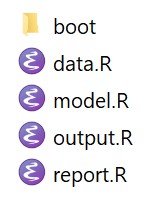
\includegraphics[width=0.12\textwidth]{explorer_1}
  \end{itemize}
\end{frame}

% ______________________________________________________________________________

\begin{frame}{Boot and Run}\small
  \begin{itemize}
    \item[] To run a TAF analysis, the first step is to start R and make sure
    that\\
    the {\green current working directory} is set to the location of the TAF
    scripts\\
    {\tt data.R}, {\tt model.R}, etc.\\[4ex]
    Some R editors do this automatically when opening an R script and\\
    in RStudio there is a menu command:\\[1ex]\it
    \qquad Session - Set Working Directory - To Source File Location\\[2ex]
    \green\sf\qquad[\:\!Alt-s w s\;\!]
  \end{itemize}
\end{frame}

% ______________________________________________________________________________

\begin{frame}{Boot and Run}\small
  \begin{itemize}
    \item[] All TAF analyses can be run using the following commands in
    R:\\[2ex]
    \begin{tt}
      \qquad{\blue library}(TAF)\\
      \qquad{\blue taf.boot}()\\
      \qquad{\blue source.all}()\\[3ex]
    \end{tt}
    \item[] The {\tt\blue taf.boot()} function looks for an existing boot folder
    to set up the\\ data and software required for the analysis.\\[3ex]
    Then {\tt\blue source.all()} runs the {\tt data.R}, {\tt model.R}
    {\tt output.R}, and {\tt report.R}\\ scripts in that order.\\[3ex]
    The individual scripts can also be run using {\tt\blue source()} or line by
    line in an\\
    R editor.\\[4ex]
  \end{itemize}
\end{frame}

% ______________________________________________________________________________

\begin{frame}{Boot and Run}\small
  \begin{itemize}
    \item[] After running the analysis, each script has created a corresponding
    folder,\\[0.2ex]
    {\tt data.R} creating a data folder, etc.\\
  \end{itemize}
  \begin{columns}[T]
    \column{0.2\textwidth}
    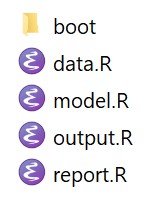
\includegraphics[width=0.6\textwidth]{explorer_1}\\
    Lorem ipsum dolor sit amet, consectetur adipisicing elit, sed do eiusmod
    tempor incididunt ut labore et dolore magna aliqua.
    \column{0.05\textwidth}
    \vspace{4ex}
    \green\large$\Rightarrow$
    \column{0.2\textwidth}
    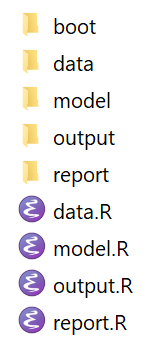
\includegraphics[width=0.6\textwidth]{explorer_2}
  \end{columns}
\end{frame}

\end{document}
